\documentclass[12pt,utf8,notheorems,compress]{beamer}
\usepackage{etex}

\usepackage[english]{babel}

\usepackage{amsmath,amssymb}
%\usepackage[framed,amsmath,thmmarks,hyperref]{ntheorem}

%\usepackage[small,nohug]{diagrams}
%\diagramstyle[labelstyle=\scriptstyle]

%\usepackage[protrusion=true,expansion=false]{microtype}

%\usepackage{lmodern}
\usepackage{tabto}
\usepackage{tikz}
\usepackage{array}
\usepackage[all]{xy}

%\usepackage[natbib=true,style=numeric]{biblatex}
%\usepackage[babel]{csquotes}
%\bibliography{lit}

%\usepackage{hyperref}

\setlength\parskip{\medskipamount}
\setlength\parindent{0pt}

%\theoremseparator{:}
\theoremstyle{plain}  %nonumberplain
%\newtheorem{beh}{Behauptung}
\newtheorem{proposition}{Proposition}
\newtheorem{corollary}{Korollar}
\newtheorem{theorem}{Satz}
\theoremstyle{definition}
\newtheorem{definition}{Definition}
%\newtheorem{kor}{Korollar}
%\newtheorem{satz}{Satz}
%\newtheorem{lemma}{Lemma}
%\newtheorem{hilfsaussage}{Hilfsaussage}
%\theorembodyfont{\normalfont}
\newtheorem{axiom}{Axiom}
%\newtheorem{defnprop}{Definition/Proposition}
%\newtheorem{bem}{Bemerkung}
%\newtheorem{bsp}{Beispiel}
%\theoremsymbol{\ensuremath{\openbox}}
%\newtheorem{proof}{Beweis}
%\newtheorem{defn}{Definition}

\newcommand{\lra}{\longrightarrow}
\newcommand{\lhra}{\ensuremath{\lhook\joinrel\relbar\joinrel\rightarrow}}
\newcommand{\thlra}{\relbar\joinrel\twoheadrightarrow}

\newcommand{\Z}{\mathbb{Z}}
\renewcommand{\C}{\mathcal{C}}
\newcommand{\N}{\mathbb{N}}
\newcommand{\R}{\mathbb{R}}
\newcommand{\Hom}{\mathrm{Hom}}
\newcommand{\id}{\mathrm{id}}
\newcommand{\Aut}[1]{\operatorname{Aut}(#1)}
\newcommand{\GL}[1]{\operatorname{GL}(#1)}
\newcommand{\freist}{\_{}\_{}}
\newcommand{\Set}{\mathrm{Set}}
\newcommand{\Grp}{\mathrm{Grp}}
\newcommand{\Vect}{\mathrm{Vect}}

\def\longleadsto{\mathrel{-}\joinrel\leadsto}
\DeclareMathOperator{\ggT}{ggT}
\DeclareMathOperator{\Ob}{Ob}
\newcommand{\op}{\mathrm{op}}

\title{Markov chains and MCMC methods}
\author[Kleine Bayessche AG]{%
  %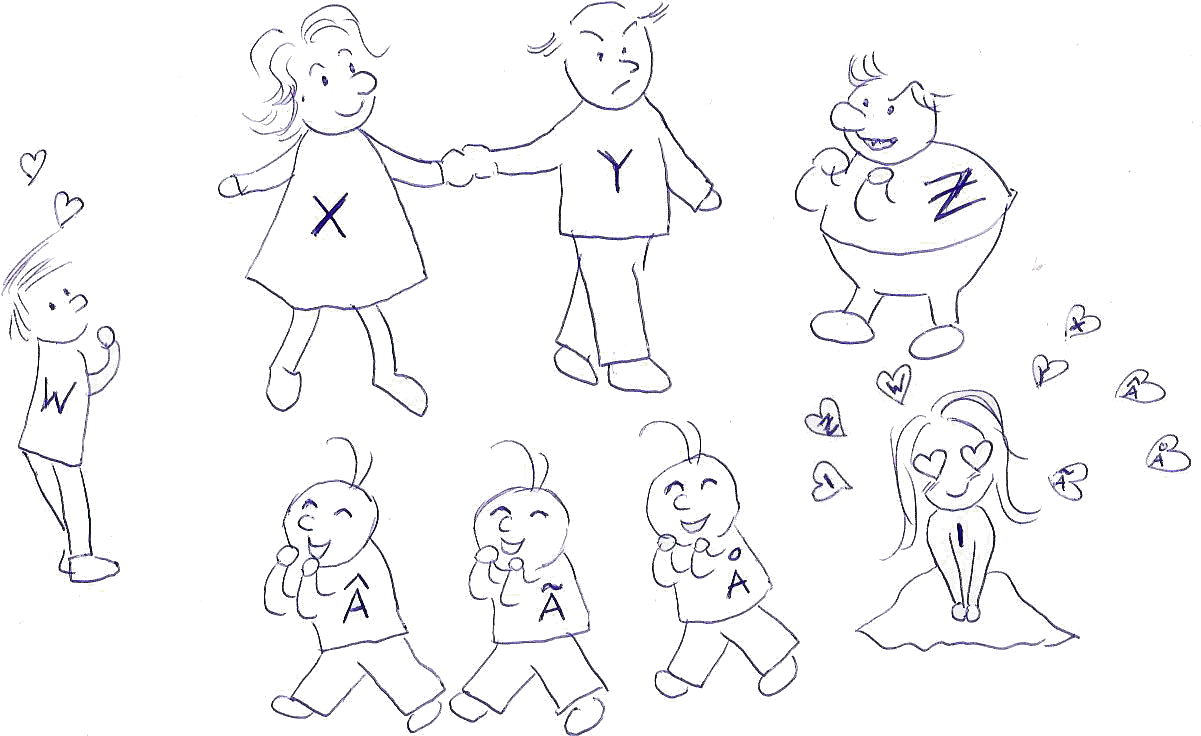
\includegraphics[scale=0.4]{relationen.png}
  }
%Ingo Blechschmidt \\ mit Illustrationen von Carina Willbold}
%\institute{Pizzaseminar in Mathematik}
\date{7. November 2014}

%\usetheme{Warsaw}  %Warsaw, Berkeley?
\usetheme{Warsaw}
\useoutertheme{split}
\usecolortheme{seahorse}
\usefonttheme{serif}
\usepackage{kurier}
\useinnertheme{rectangles}
%\usepackage{bookman}
%\setbeamercovered{transparent}

\setbeamertemplate{navigation symbols}{}
%\setbeamertemplate{footline}{}
%\setbeamertemplate{headline}{}

%\beamertemplateboldcenterframetitle
%\setbeamerfont{frametitle}{size={\Large}}

\newcommand*\oldmacro{}%
\let\oldmacro\insertshorttitle%
\renewcommand*\insertshorttitle{%
  \oldmacro\hfill\insertframenumber\,/\,\inserttotalframenumber\hfill}

\newenvironment{changemargin}[2]{%
  \begin{list}{}{%
    \setlength{\topsep}{0pt}%
    \setlength{\leftmargin}{#1}%
    \setlength{\rightmargin}{#2}%
    \setlength{\listparindent}{\parindent}%
    \setlength{\itemindent}{\parindent}%
    \setlength{\parsep}{\parskip}%
  }%
  \item[]}{\end{list}}

\newcommand{\hil}[1]{{\usebeamercolor[fg]{item}{#1}}}

\begin{document}

\setbeameroption{show notes}
\setbeamertemplate{note page}[plain]

\frame{\titlepage}
%\frame[t]{\frametitle{Gliederung}\begin{minipage}{\textwidth}\begin{small}\tableofcontents\end{small}\end{minipage}}
\frame[t]{\frametitle{Outline}\tableofcontents}

\section[Chat bot]{Live demo: an IRC chat bot}

\frame{
  \begin{center}
    \huge
    Live demo: an IRC chat bot
  \end{center}
}


\section[Basics]{Basics on Markov chains}

\frame[t]{\frametitle{What is a Markov chain?}
  \begin{itemize}
    \item A Markov chain is a system which undergoes transitions from one state
    to another according to probabilities~$P(X' = j \,|\, X = i) =: p_{ij}$.
    \vfill
    \item More abstractly, a Markov chain on a state space~$S$ is a map~$S \to
    D(S)$, where~$D(S)$ is the set of probability measures on~$S$.
    \vfill
    \item Categorically, a Markov chain is a coalgebra for the functor~$D :
    \Set \to \Set$.
  \end{itemize}
}

\note{
  The following systems can be modeled by Markov chains:
  \begin{itemize}
  \item the position of a peg in the game of snakes and ladders
  \item the position of a random walk
  \item the weather, if we oversimplify a lot
  \end{itemize}

  The following cannot:

  \begin{itemize}
  \item the state of a game of blackjack
  \end{itemize}
}

\frame[t]{\frametitle{Basic theory on Markov chains}
  \begin{itemize}
    \item Transition matrix is a stochastic matrix
    \item Main theorem
    \item XXX
  \end{itemize}
}

\section[Sampling]{Sampling from distributions}
\frame[t]{\frametitle{How can we sample from distributions?}
  Given a density~$f$, want independent samples~$x_1,x_2,\ldots$
  \bigskip

  \only<1-2>{\begin{itemize}
  \item<1-2> If the inverse of the cumulative distribution function~$F$ is available:
  \bigskip

        \begin{enumerate}
        \item Sample~$u \sim U(0,1)$.
        \item Output~$x := F^{-1}(u)$.
        \end{enumerate}

  \bigskip
  \item<2> Unfortunately, calculating~$F^{-1}$ is expensive for general
  densities~$f$.\end{itemize}}

  \begin{itemize}
  \item<3,4> If some other sampleable density~$g$ with $f \leq M g$ is
  available, can use \hil{rejection sampling}:
  \bigskip

  \begin{enumerate}
  \item Sample~$x \sim g$.
  \item Sample~$u \sim U(0,1)$.
  \item If~$u < \frac{1}{M} f(x)/g(x)$, output~$x$; else, retry.
  \end{enumerate}

  \bigskip
  \item<4> Works even if~$f$ is only known up to a constant factor.
  \item<4> Acceptance probability is~$1/M$, this might be small.
  \end{itemize}
}

\note{
  \fontsize{8pt}{9.6}\selectfont
  \begin{itemize}
    \item Proof that the easy sampling algorithm is correct:
          \[ P(F^{-1}(U) \leq x) = P(U \leq F(x)) = F(x). \]

    \item Acceptance probability in rejection sampling:
          \begin{align*}
            P(U < \tfrac{1}{M} f(Q)/g(Q)) &=
             E(\tfrac{1}{M} f(Q)/g(Q)) \\&=
             \tfrac{1}{M} \cdot \int f(x)/g(x) \cdot g(x) \,dx =
             \tfrac{1}{M}.
          \end{align*}
    \item Proof of correctness:
          \begin{align*}
            P(G \leq x \,\wedge\, U < \tfrac{1}{M} f(G)/g(G))
            &= \int P(G \leq x \,\wedge\, U < \tfrac{1}{M} f(G)/g(G) \ |\ G = t) g(t)\,dt \\
            &= \int \boldsymbol{1}_{t \leq x} \cdot P(U < \tfrac{1}{M} f(t)/g(t)) \cdot g(t) \,dt \\
            &= \int \boldsymbol{1}_{t \leq x} \cdot \tfrac{1}{M} f(t)/g(t) \cdot g(t) \,dt \\
            &= \tfrac{1}{M} F(x), \\[1em]
            \text{so}\quad P(G \leq x \ |\ U < \tfrac{1}{M} f(G)/g(G)) &= F(x).
          \end{align*}
  \end{itemize}
}

\frame[t]{\frametitle{Markov chain Monte Carlo methods}
  Given a density~$f$, want independent samples~$x_1,x_2,\ldots$

  \begin{enumerate}
    \item Construct a Markov chain with limiting distribution~$f$.
    \item Draw samples from the chain.
    \item Discard first samples (burn-in period).
    \item From the remaining samples, retain only every~$N$'th.
  \end{enumerate}

  Works very well in practice.
}

\frame[t]{\frametitle{Metropolis--Hastings algorithm}
  Given a density~$f$, want independent samples~$x_1,x_2,\ldots$

  Let~$g(y,x)$ be such that for any~$x$, $g(\cdot,x)$ is sampleable.
  Set~$B(x,y) := \frac{f(y) g(x,y)}{f(x) g(y,x)}$ and~$A(x,y) := \min\{1,\,A(x,y)\}$.

  \begin{enumerate}
    \item Initialize~$x$.
    \item Sample~$u \sim U(0,1)$.
    \item Sample~$y \sim g(\cdot,x)$.
    \item If~$u < A(x,y)$, set~$x := y$.
    \item Output~$x$ and go back to step~2.
  \end{enumerate}

  Works even if~$f$ and~$g$ are only known up to constant factors.
}

\note{
  \begin{itemize}
    \item Transition matrix (really, kernel):
    \[ T(x,y) = \hat g(y,x) A(x,y) + \delta(x,y) \int (1-A(x,z)) \hat g(z,x) \,dz. \]

    \item Balance condition (for~$x \neq y$):
    \[ f(x) T(x,y) = \min\{ f(x) \hat g(y,x),\, f(y) \hat g(x,y) \} =
      f(y) T(y,x). \]
  \end{itemize}
}

\section[Integrals]{Evaluating integrals over high-dimensional domains}
\frame[t]{}

\end{document}
